\documentclass[10pt,draftclsnofoot,onecolumn,compsoc]{IEEEtran}
\usepackage[letterpaper, portrait, margin=0.75in]{geometry}
%\usepackage[myheadings]{fullpage}
\usepackage{fancyhdr}
\usepackage{lastpage}
\usepackage{graphicx,  subcaption,  booktabs}
\usepackage[T1]{fontenc}
\usepackage[font=small, labelfont=bf]{caption}
%\usepackage{fourier}
\usepackage[protrusion=true, expansion=true]{microtype}
\usepackage[english]{babel}
%\usepackage{sectsty}
\usepackage{url, lipsum}
\usepackage{tikz}
\usepackage[section]{placeins}
\usepackage{makeidx}
\newcommand{\subparagraph}{}
\usepackage{titlesec}

\makeatletter
\renewcommand{\@IEEEsectpunct}{ \\ \\ \,}% Modified from {:\ \,}
\makeatother

\setlength{\parindent}{0em}
\setlength{\parskip}{1em}
\renewcommand\thesection{\arabic{section}}
\renewcommand\thesubsection{\thesection.\arabic{subsection}}
\renewcommand\thesubsubsection{\thesubsection.\arabic{subsubsection}}

\makeatletter
\renewcommand\paragraph{\@startsection{paragraph}{4}{\z@}%
                                    {0ex \@plus0ex \@minus.0ex}%
                                    {0em}%
                                    {\normalfont\normalsize\bfseries}}
\makeatother

\renewcommand\thesectiondis{\arabic{section}}
\renewcommand\thesubsectiondis{\thesectiondis.\arabic{subsection}}
\renewcommand\thesubsubsectiondis{\thesubsectiondis.\arabic{subsubsection}}


\titleformat{\section}
       {\normalfont\fontfamily{phv}\fontsize{14}{17}\bfseries}{\thesection}{1em}{}
\titleformat{\subsection}
       {\normalfont\fontfamily{phv}\fontsize{14}{17}\bfseries}{\thesubsection}{1em}{}
\titleformat{\subsubsection}
       {\normalfont\fontfamily{phv}\fontsize{14}{17}\bfseries}{\thesubsubsection}{1em}{}


\newcommand{\namesigdatehrule}[1]{\par\tikz \draw [blue, densely dotted, ultra thick] (0,0) -- (#1,0);\par}
\newcommand{\namesigdate}[2][5cm]{%
\begin{minipage}{#1}%
    #2 \vspace{0.8cm}\namesigdatehrule{#1}\smallskip
    \small \noindent\textit{Signature}
    \vspace{0.8cm}\namesigdatehrule{#1}\smallskip
    \small \textit{Date}
\end{minipage}
}


\newcommand{\HRule}[1]{\rule{\linewidth}{#1}}
\newcommand*\tick{\textsc{\char13}}
\linespread{1}
\setcounter{tocdepth}{5}
\setcounter{secnumdepth}{5}

\makeindex

\begin{document}
%\title{HyRo (Working title)}
%\author{Jason Klindtworth  |  Josh Asher  |   Layne Nolli}
%\date{}
%\maketitle
\begin{titlepage}
	\centering
	{\scshape\LARGE HyRo \par}
	%\vspace{1cm}
	{\scshape\LARGE Team 28\par}
	\vspace{1cm}
	{\scshape\Large Jason Klindtworth  |  Josh Asher  |   Layne Nolli}
	\noindent\makebox[\linewidth]{\rule{17cm}{2pt}}
	\vspace{1cm}
	{\huge\bfseries CS461\par}
	\vspace{2cm}
	{\Large\itshape Fall 2016\par}
	\vspace{4cm}
	{\large Requirements Document\par}\vspace{8cm}
	\noindent\makebox[\linewidth]{\rule{17cm}{2pt}}
	\vfill

% Bottom of the page
	{\large \today\par}
\end{titlepage}

%\newpage
%\sectionfont{\scshape}
%\title{Abstract}

\setcounter{tocdepth}{2}
\tableofcontents

\section{ Introduction}
%\sectionfont{\scshape}
\subsection{Purpose}
\index{Purpose}
  This document contains the software requirements that describe components of a system for a hybrid rocket that will communicate instructions, retrieve data, log commands,
 visualize data, and visualize controls for such a rocket.  This document will provide scope, definitions, an overall description, and specific requirements for this system.
 This system will be used by the OSU Hybrid Rocket team to launch and visualize data from their rocket. Persons involved include Nancy Squires, ME Senior Students, ECE senior students,
 and other rocket club members that have chosen to be part of this team. Our audience members have an inclination to participate in rocketry. The system will be part of the ESRA
competition and has a potential to be recognized by the AIAA who support this competition.
\subsection{Scope}
\index{Scope}
 There are 2 separate components to this avionics system. 

\subsubsection{HyRo OS}
\index{HyRo OS}
HyRo OS is a program residing on a Beagle Bone Black embedded Linux computer that will be onboard the hybrid rocket. This software component will collect sensor and possibly
 GPS data from onboard electrical components and send this data to the ground team. HyRo OS is also responsible for receiving rocket commands from the ground team and responding to those
 commands by sending electrical signals to appropriate onboard electrical equipment. The purpose of this component is to provide reliable communication to the ground team for commanding
the rocket and gathering its data. 
\subsubsection{HyRo VS}
\index{HyRo VS}
HyRo VS is software residing on a traditional computer that will send and receive data and commands to the rocket's onboard HyRo OS component. HyRo VS will be the ground teams graphical interface for data visualization, logging, and issuing commands to the system. It will present the ground team with input buttons to issue appropriate commands and data visualization windows to monitor data transferred from the hybrid rockets on board HyRo OS. This software will benefit the ground team by providing data visualization from the hybrid rocket that previously was not human readable. It also will provide command input into the system that benefits the ground team by ease of use and safety.

\subsection{Definitions, acronyms, and abbreviations}
\index{Definitions, acronyms, and abbreviations}
\subsubsection{\bf ESRA:}  The Experimental Sounding Rocket Association is a non-profit organization founded in 2003 for the purpose of fostering and promoting engineering in rocketry.
\subsubsection{\bf AIAA:} The American Institute of Aeronautics and Astronautics is the world's largest technical society dedicated to the global aerospace profession.
\subsubsection{\bf Avionics System:}  A system for controlling launch and other system function on a rocket, along with collecting data from onboard sensors.
\subsubsection{\bf Onboard:} Any component of the system that is housed in the rocket chassis.
\subsubsection{\bf Beagle Bone Black(BBB):}   A micro controller running Debian Linux connected to onboard components of the rocket.
\subsubsection{\bf HyRo OS:}  The HyRo rocket team's onboard operating system.
\subsubsection{\bf HyRo VS:} The HyRo rocket team's command and visualization software running on a traditional computer.
\subsubsection{\bf Embedded:} A software system that is running on microcontroller with no visual output.
\subsubsection{\bf Hybrid Rocket:} A rocket that has both solid fuel and liquid fuel. This creates the ability to throttle the rocket's motor.
\subsubsection{\bf GPS:} Global position satellite. In the aspect of this paper, a sensor that collects positional data in relation to the earth. This data is formatted for use in GPS applications to visualize the location of the sensor.
\subsubsection{\bf Ground Team:} The group of rocket team members controlling the rockets operation and viewing its data. Located a distance from the launch site on the ground.
\subsubsection{\bf Traditional Computer:}A computer, like a laptop, running an operating system. The operating system we will consider are Windows or Linux.
\subsubsection{\bf Remote Filling:} Filling the oxidizer from a safe distance via commands from the ground team.
\subsubsection{\bf Arming:} Preparing the rocket to ignite.
\subsubsection{\bf Disarming:} Reversing the rockets arming condition. 
\subsubsection{\bf Launch:} Releasing the rocket into the skies! 
\subsubsection{\bf Abort:} Completely stopping the rockets launching operations.
\subsubsection{\bf Ignition:} Starting the rocket motors combustion process.
\subsubsection{\bf Liquid Oxidizer:}Liquid part of the rockets fuel. 
\subsubsection{\bf Oxidizer Tank:} Tank were the liquid oxidizer is held. 
\subsubsection{\bf Chamber:} Where the two fuels mix.
\subsubsection{\bf PSI:}Pounds per square inch. A unit measuring pressure. 
\subsubsection{\bf Pa:} Pascals. A unit measuring pressure.
\subsubsection{\bf PWM:} Pulse Width Modulation - An electronic control signal used to change state of electrical components.
\subsubsection{\bf GPIO:}  General Purpose Input Output lines are used to communicate to sensors and electronic components.
\subsubsection{\bf SPI:}  Serial Peripheral Interface - A protocol to communicate with micro controllers.
\subsubsection{\bf I2C:}  Inter-Integrate Circuit - A protocol to communicate with micro controllers.
\subsubsection{\bf OS:} Operating System - the main system running on a micro controller or a traditional computer.
\subsubsection{\bf LSM9DS0:} The LSM9DS0 is a system-in-package featuring a 3D digital linear acceleration sensor,  a 3D digital angular rate sensor, and a 3D digital magnetic sensor.
\subsubsection{\bf TGY6114MD:}A powerful high specification digital sail winch servo with metal gears that can be programmed to operate from 1 to 6 turns.
\subsubsection{\bf BM180:}Digital pressure sensor.
\subsubsection{\bf API:}An application program interface is a set of routines, protocols, and tools for building software applications. An API specifies how software components should interact.
\subsubsection{\bf RAM:}Random Access Memory
\subsubsection{\bf Gauge:}A graphical device to display the readout of a sensor. For example a speedometer.
\subsubsection{\bf Serial Communication:}Data sent back to back through a medium.

\subsection{ References}
Beagle Bone Black hardware specifications from elinux.org [http://elinux.org/Beagleboard:BeagleBoneBlack]\\
BMP180 Digital Pressure Sensor data sheet [https://cdn-shop.adafruit.com/datasheets/BST-BMP180-DS000-09.pdf]\\
LSM9DS0 3D accelerometer, 3D gyroscope, 3D magnetometer data sheet http://www.st.com/content/ccc/resource/technica\\l/document/datasheet/ab/2a/3b/45/f0/92/41/73/DM00087365.pdf/files/DM00087365.pdf/jcr:content/translations\\/en.DM00087365.pdf]
\index{References}
\subsection{Overview}
\index{Overview}
The rest of this document contains over all descriptions of the different components of this system. Followed by specific requirements of these components.

\section{ Overall Description}
\index{Overall Description}
\subsection{ Product perspective}
\index{Product perspective}
Our software components are part of the overall system of the Hybrid Rocket. These components encompass remotely filling, arming/disarming, aborting, ignition, recovery, throttling, gathering sensor data, and radio communication circuitry.  On the traditional computer they encompass serial communication to the ground control unit, user input, and user data visualization. Our software will need to interface with an external GPS system if this stretch goal is reached. 

\subsubsection{System Interfaces}
\index{System Interfaces}
The HyRo VS component of our system will house the user interface to our system. This interface will be divided into a command menu, system diagnostics/status window, and different visualization windows with options on how to display the data. The full graphical user interface will fill the entire screen. The command menu will house six buttons with the potential for more to be added if necessary. All commands have not been decided on because the rocket has yet to be made and requirements and commands may be presented to our system as other teams design their parts of the hybrid rocket.  The six buttons that are required at the moment are: Arm Rocket, Disarm Rocket, Fill Liquid Oxidizer, Launch, Abort Launch, and Ignition. The command menu will be located to the left of the screen and take up approximately 1/4 the width of the screen and approximately 1/2 the height of the screen. Buttons in the menu will be evenly spaced and use around a size 20pt font for text inside the buttons. \par
	Under the command menu on the left hand side of the screen will be the system diagnostics and status window. This window will take up 1/4 the width of the screen and 1/4 the height of the screen. This screen will report status of the various system components including indication of functioning communication between the hybrid rocket, the ground control unit, and the system which this software resides on. It will also include the state of the rocket (i.e. armed, disarmed, filled, etc) and any diagnostic information from sensors on the various components of the system. Exact diagnostic items have not been determined because the Hybrid Rocket has not been mechanically or electrically designed yet. These will be added to this document when the system is further along.\par 
	Under the status window will be a graphing window options menu. This will take up 1/4 the width of the screen on the left and 1/4 its height. From this menu a user can select if they would like to individually look at larger graph of a particular piece of data. \par
	The visualization windows will be housed in a parent container that will encompass 3/4 of the screen width and the total height of the screen. There is a total of 7 different groups of data that need to be visualized.  If any more sensors are added to this system once it is developing these will be added to this document with and explanation as to how they will be visualized.  The current group of data to be visualized includes:  Oxidizer tank pressure, chamber pressure, Oxidizer tank temperature, acceleration, barometric pressure, velocity, and GPS.   Each individual item might be represented as a gauge or graph.\par
	
The visualization units have not fully been determined and are listed as options until further development of the hybrid rocket occurs and we have feedback from the rest of the team as to what units will be the most appealing. Users will have the option to either graph the data or display the data in gauge format with a needle pointing to the current value of that data. \par


\begin{figure}
  \caption{Basic Mock Up of User Interface for Hyro showing implementation of UI layout and positioning of objects like buttons, graphs, and dials for the user to process at a glance. This is a test mock up and may not be exact to the final product. }
  \centering
	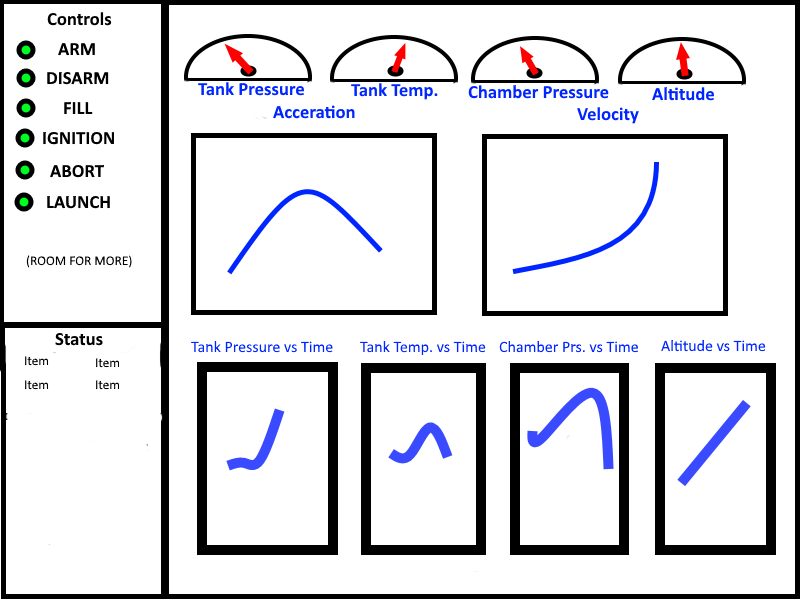
\includegraphics[scale=.75]{HyRoUIMockup}
\end{figure}
\index{User Interface Mockup}
\FloatBarrier
\subsubsection{Hardware Interfaces}
\index{Hardware Interfaces}
Each of the three components to our software will require specific interfaces to different hardware aspects depending on which part of the system they are located in.\par

{\bf HyRo OS}
 	HyRo OS will be connected to the onboard electrical systems of the rocket. These systems include sensors that collect data, servos that control various action internal to the rocket, a radio frequency transmitter for communication, and any other electrical device critical to the rockets operation. Many of these components have yet to be determined and will be conceived next term when work begins on the mechanical and electrical aspects of the rocket.  We do know all sensors on board the rocket from last year have pre-built interfaces that can connect to the BBB using common electrical protocols like I2C or SPI. They come with an API that can be used on the BBB to access their data. . Servos and other electrical components will use PWM lines available on the BBB to communicate desired functionality. The radio module used communicates to the BBB via serial communication. All the GPIO, PWM, and Serial lines on the BBB are interfaced through its operating system and come pre-configured for API access.\par

{\bf HyRo VS}
HyRo VS will need to communicate to a serial port on the computer it is residing on.  This will be done through either a Windows or Linux serial port access API.

\subsubsection{Software Interfaces}
\index{Software Interfaces}
	We will be interfacing various outside software products. These include the Debian Linux operating system running on the BBB, the Operating system running on the traditional computer which will be either Linux or Windows and possibly an external GPS program which is part of our stretch requirements.

\subsubsection{Communication Interfaces}
\index{Communication Interfaces}
There are two interfaces for communication in our system and both require the use of a serial interface. The first is radio communication with a radio frequency transceiver. There will be one onboard the rocket connected to the BBB and one connected to the traditional computer via a USB interface. The serial communication is accessed through an API and acts like a file descriptor. We will design a protocol to transfer commands and data over these serial interfaces. Each command will have a name and parameters associated with it. Data will have a name associated with it followed by the actual data.

\subsubsection{Memory Constraints}
\index{Memory Constraints}
The HyRo VS aspect of our system will be constrained by the memory of the traditional computer it is located on. Available memory should be significant enough that we should not be constrained. This is because our program will have a small footprint and the data we log will not exceed 200 megabytes.\par 
	The HyRo OS will be constrained to 512 megabytes of RAM and 4 Gigabytes of onboard long term memory. Our onboard system will need to be able to run in the RAM available and not store over 4 gigabytes of data.


\subsubsection {Operations}
\index{Operations}
There are 4 modes of operation in our system: pre-launch, staging, in flight, and post flight.  Pre-launch operations will be non-interactive and display status of the system components. The system will process data relating to the status of onboard components and display them in the status window. All buttons will be highlighted in a color corresponding to their status. We will have a background system monitoring all input from the control mechanism sent through the serial communication. \par
	Staging will be an interactive process where the user will provide input to various command buttons. The buttons will have to be executed in order, except for the abort button. Components will monitor user input and prime the ignition system as defined by the ignition sequence. These functions will not allow user input in the wrong order. If the abort command is issued all other function will be overridden and the system will return to its pre-launch state. Once the sequence has been completed the software will switch to the in-flight mode. A support function that logs all commands to a log file will be implemented to record these actions.\par
	The in-flight mode will disable the command menu and begin data collection from the onboard sensors. At this point all sensor data processing function will be activated. The data will be received from the serial port, parsed through the data processor, and sent to the appropriate data processing functions. These functions are responsible for visualizing the data on our graphs and gauges. These operations are to be monitored by the user for visual satisfaction.  The data will also be logged by a logging function in a text format to be used by the post-flight mode.
	Post flight mode will be fully interactive. The command menu will still be disabled but data stored by the data logger will be able to be viewed in graphs that related the data over time of flight. These graphs will be viewable by selecting them from the data menu and expressing which data items you would like to see a graph of. \par

\subsubsection{Site Adaption Requirements}
\index{Site Adaption Requirements}
When the hybrid rocket is ready to launch the software will be in pre-launch mode and a sequence of commands must be sent to the rocket in order for the rocket to be safely launched. This sequence is fill, arm, ignite, and launch. At any moment someone can cancel this sequence if the rocket is deemed not safe to launch by using the abort button.

\subsection{ Product functions}
\index{Product functions}
Our software as a whole will function as a way to communicate information from the hybrid rocket to a traditional computer on the ground. The ground team will interact with the ground computer to look at the information from the rocket and pass information back to the rocket. Both software components each have their own unique functions.

\subsubsection{HyRo OS}
\begin{itemize}
\item Send and Receive communications from a radio transceiver to communicate with the ground team.
\item Collect sensor data from any onboard sensors when in flight.
\item Send sensor data to the ground computer.
\item Monitor fill and launch systems and send information to ground team.
\item Receive commands from ground team.
\item Send electrical signals or messages to launching components when appropriate command is received.
\item Make sure commands are executed in correct order.
\item Send signal to deploy chute at correct altitude.
\end{itemize}

\subsubsection{HyRo VS}
\begin{itemize}
\item Send and Receive communication from a radio transceiver to communicate with the hybrid rocket.
\item Provide a status view so team can monitor onboard rocket components.
\item Provide a menu of commands to stage, launch, or abort the rocket mission.
\item Log all commands that have been sent.
\item Collect data sent from the rocket and store it.
\item Collect data from the rocket and visualize it on the screen in its appropriate gauge or graph while rocket is in flight.
\item Provide a log of the data.
\item Provide the ability to view different categories of data in a graph with a menu for the user to choose what data from the flight they would like to view.\end{itemize}

\begin{figure}[!ht]
\index{Data Flow Diagram of HyRo}
  \caption{Data Flow Between System Components.}
  \centering
	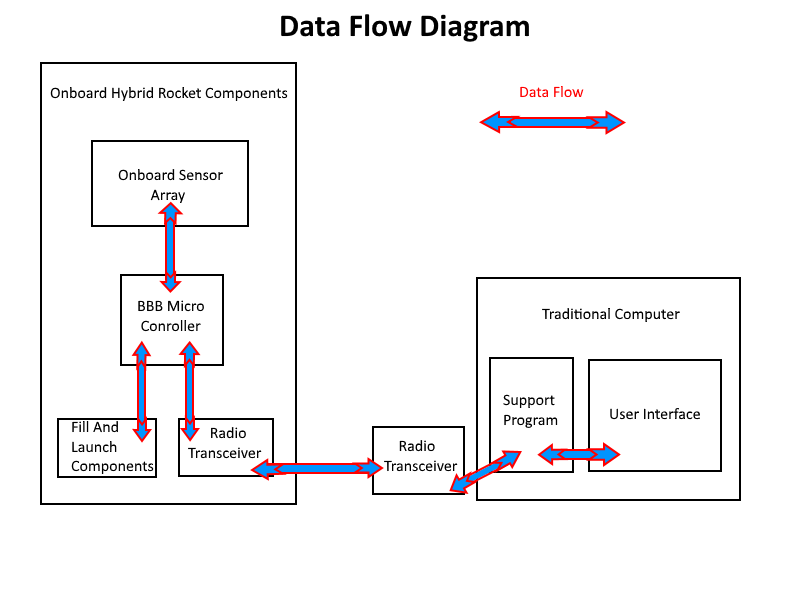
\includegraphics[scale=.85]{RocketBlockDiagram}
\end{figure}
\FloatBarrier
\subsection{ User characteristics}
\index{User characteristisc}
Intended users of this software require a knowledge of rocketry and safe handling of launching a rocket. These users will be undergraduate students, graduate students, and professors included in the rocket team. They will have sufficient knowledge of the operation and safety requirements of launching a hybrid rocket according to the safety regulation of ESRA.

\subsection{Constraints}
\index{Constraints}

\index{Regulatory Policies}
\subsubsection{\bf  Regulatory Policies}Operation of our software must stay in the bounds set by ESRA and the safe handling and operation of launching a hybrid rocket.  

\index{Hardware Limitations}
\subsubsection{\bf Hardware Limitations} HyRo OS will be onboard a BBB with only 512 megabytes of ram and 4 gigabytes of storage and must function under these restrictions. The BBB will also be inside of a volatile environment inside the rocket that could cause it to overheat. Timing is also a major concern in communicating sensor data and commands. All communication between the rocket, its sensors, its launching components, and the ground team must be within 1  second or less.

\index{Interfaces to other applications}
\subsubsection{\bf  Interfaces to other applications} If GPS is used we will have to output data to a GPS application in the correct format for that application.
\index{Control Functions}
\subsubsection{\bf Control Functions} Launching of the rocket must be monitored in the correct order or our software should not continue the sequence to launch the rocket.
\index{Reliability Requirements}
\subsubsection{\bf Reliability Requirements} Data in our system must be transferred and interpreted in a complete and reliable fashion. Incomplete commands will be ignored. Incomplete sensor data will also be ignored. Data loss will not exceed 10 percent or our system will not be reliable.
\index{Safety Considerations}
\subsubsection{\bf Safety Considerations} Our software must not stage and launch the rocket without receiving the appropriate sequence of commands from the ground team. Failure to do so may result in harm to team members.

\subsection{Assumptions and dependencies}
\index{Assumptions and dependencies}
Our onboard software system HyRo OS assumes that it will be installed on a Debian Linux OS that is running on a BBB.  HyRo OS assumes it will be connect to a XBee radio transceiver, a TGY6114MD servo, a LSM9DS0 accelerometer/gyroscope, and a BMP180 Barometric pressure altitude sensor.\par
	Our HyRo VS software running on a traditional computer assumes that it will be communicating with a XBee radio transceiver.

\subsection{Apportioning of Requirements}
\index{Gantt Chart for HyRo}
\begin{figure}
  \caption{Gantt chart for HyRo Workflow over the course of the project. This chart is highlighting overlapping responsibilities between team members that are broken into manageable chunks to ensure time management. }
  \centering
	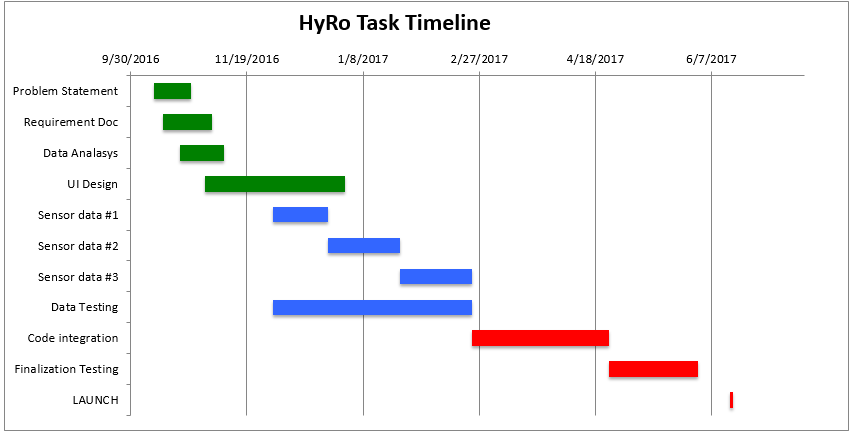
\includegraphics[scale=.75]{GanntChart}
\end{figure}
\FloatBarrier
\subsubsection{\bf GPS - (Stretch Goal)} A GPS sensor might be installed on the rocket. This will require the HyRo OS to be able to communicate with this sensor and transmit its data. The HyRo VS then will need to be able to collect this data and either display it in a GPS window of our design or pass it onto to a GPS application that will interpret the data to find the rockets location.
\subsubsection{\bf Throttling - (Stretch Goal)} If the system is stable in time the team would like to be able to automatically throttle the rocket in flight. Throttling will enable the rocket to reach a higher altitude. The HyRo OS will need to make inflight calculations and adjust the Oxidizer valve to the appropriate throttling level. This will require advanced math calculations and accurate valve adjusting.

\section{ Specific requirements}
\subsection{External Interface Requirements}
\index{User Interface Requirements}
\subsubsection{ User Interfaces}
\index{User Interfaces}
\paragraph {\bf Fill Command Button Input}
\index{Fill Command}
The fill command input button will activate the fill servo to fill the chamber with oxidizer. This command is inputted from a button on the command menu. The command will be formatted in an English representation.  This command must be sent within 1 second. This command must be sent before the arming command is given. Other commands will not function out of this sequence. It will be located in the command menu of the left hand side of the screen.

\paragraph{\bf Arming Command Button Input}
\index{Arming Command}
The arming command input button will send a command to the system that will arm the rocket. This command is inputted from a button on the command menu. The command will be formatted in an English representation.  This command must be sent within 1 second. This command must be sent before the ignition command is given. Other commands will not function out of this sequence. It will be located in the command menu of the left hand side of the screen.

\paragraph{\bf Ignition Command Button Input}
\index{Ignition Command}
The ignition command input button will activate the ignition system of the rocket. This command is inputted from a button on the command menu. The command will be formatted in an English representation.  This command must be sent within 1 seconds. This command must be sent before the launch command is given. Other commands will not function out of this sequence. It will be located in the command menu of the left hand side of the screen.

\paragraph{\bf Launch Command Button Input}
\index{Launch Command}
The launch command input button will release the rocket when it is ignited. This command is inputted from a button on the command menu. The command will be formatted in an English representation.  This command must be sent within 1 second. This command must be sent last in the sequence of commands. Other commands will not function out of this sequence. It will be located in the command menu of the left hand side of the screen.

\paragraph{\bf Disarm Command Button Input}
\index{Disarm Command}
The disarm command input button will disable the arming of the rocket. This command is inputted from a button on the command menu. The command will be formatted in an English representation.  This command must be sent within 1 second. This command can be issued anytime the rocket has been armed. It will be located in the command menu of the left hand side of the screen.

\paragraph{\bf Abort Command Button Input}
\index{Abort Command}
The abort command input button will return the system to its pre-launch state and stop the rocket from launching. This command is inputted from a button on the command menu. The command will be formatted in an English representation.  This command must be sent within 1 second. This command can be issued at any time and is not effected by other command buttons. It will be located in the command menu of the left hand side of the screen.

\paragraph{\bf Command Output to radio transceiver}
\index{Command Output}
	Any time a command is received from the command menu the HyRo VS will send the command to the radio transceiver. The UI for the commands will all be formatted in plain English. Commands must be delivered in under 1 second.

\paragraph{\bf System Status Input}
\index{System Status Input/Output}
	The system status input receives status data from the radio transceiver to be passed to the user interface. The status will be formatted with the item name appended by the status data from that part of the system. Status messages will be delivered in under 1 second. 

\paragraph{\bf System Status Output}
The system status output places the status data from the status input onto the user interface. This will be done as soon as the data is received. The status will be displayed under the command menu on the left side of the screen. We will display the system components name and the data we received together to inform the ground team the status of that rocket component.

\paragraph{\bf Sensor Data Input}
\index{Sensor Data Input/Output}
The sensor data input shall receive data from the radio transceiver to be output to the user interface. Each sensor will have its own respective units of measurement, that will be predetermined in the software, once sensors have been finalized. Data will be sent in raw form and need to be converted using predetermined conversion formulas for that particular sensor. Accuracy depends on the accuracy of the sensor that the data came from. Each input will be related to its respective graphical output in the user interface. The data will be formatted with a respective sensor name append by the data from that part of the sensor.

\paragraph{\bf Sensor Data Output}
The sensor data output will convert the data into a graph and display it on the user interface. It will have received this data from the sensor input. The data will either be graphed on a normal x-y-graph or adapted onto a gauge with a needle indicating current levels of the data within a range. The range will depend on the type of data received and be preprogrammed in the software. Units will depend on which sensor supplied the data. Each graph or gauge will take up a section of the right hand window of the user interface in its appropriate sub window. 


\subsubsection{Hardware interfaces }
\index{Hardware interfaces}
\paragraph{\bf Radio Transceiver Input/Output}
\index{Radio Transceiver Input/Output}
		Both software components will have an interface to their respective radio transceivers that will support data transfer between the rocket and the traditional computer. Any commands or data received from the various input sources will be placed onto this interface to be transmitted to the other radio transceiver. Data will be formatted with an English name representing what input it came from appended by the actual data.

\paragraph{\bf Sensor data Input}
\index{Sensor Data Hardware Input}
Sensor data input will be received from the various sensors on the system to be transmitted to the ground teams user interface. Accuracy of data depends on the accuracy of the sensors and the ability of the radio transceivers to communicate entire data package. When sensor data is inputted it is packaged and transmitted to the radio transceiver. Data format will be dictated by the format of the sensor output that has yet to be determined.

\paragraph{\bf Launch Control Electronics Input/Output}
\index{Launch Control Electronics}
This interface will monitor input from the electronic controls of the system and output their status to the radio transceiver. Data format of this part will be component name appended by the state of the component. Commands will be received to change the state of these components and appropriate electronic signal will be outputted to corresponding electronic components. Timing is critical and input and output must be performed in under 1 second.


\subsubsection{Software Interfaces}
\index{Software Interfaces}
\index{Linux OS Interface}
\paragraph{\bf Linux OS Interface}This interface will need to connect to the operating systems file descriptors and GPIO lines in order to communicate to sensors and electronics components. Inputs will be from OS and API interfaces to the operating system. These are prepackaged and will be connected to in software. Components will need to connect to the OS interfaces within 1 second. 

\subsubsection{Communication Interfaces}
\index{Communication Interfaces}
\index{Serial Communcation Interface}
\paragraph {\bf Serial Communication Interface}All communication except for to the electronic launch components will be done via serial ports. Input and Output to these port act like file descriptors and will be read and written too in such a manner. Serial communication encompasses sensor input, data output, and command input and output.

\subsection{Functions}
\index{Functions}
\subsubsection{Command Input}
\index{Command Input}
	\paragraph{ Requirement 1}Inputs must be done in previously mentioned sequence or are otherwise considered invalid. \par
	\paragraph{ Requirement 2}If command is not delivered user will have to repeat the command input.\par
	\paragraph{ Requirement 3}If the rocket components are not ready for a particular input, the command will be ignored. \par
\subsubsection{Command Output}
\index{Command Output}
	\paragraph{ Requirement 1}Sequence of the command will be checked before output.\par
	\paragraph{ Requirement 2}Command will be check against programmed commands to make sure that is valid.\par
	\paragraph{ Requirement 3}If a command is received out of sequence or is invalid the system will report back to the user interface that the command could not be completed.\par
	\paragraph{ Requirement 4}If a command is successfully output, status is returned to user interface to allow for next command to be inputted.\par

\subsubsection{Status Input}
\index{Status Input}
	\paragraph{ Requirement 1}Status input will be checked for completeness of status packet size to make sure that it is valid.\par
	\paragraph{ Requirement 2}If status input is missing no status data will be transferred and the user interface will receive a message stating the status could not be processed.\par
	\paragraph{ Requirement 3} If status message is intact it will be sent to the status output.\par
\subsubsection{Status Output}
\index{Status Output}
	\paragraph{ Requirement 1}Data will be checked for validity if it is out of bounds data will not be output to the user interface.\par
	\paragraph{ Requirement 2}Valid data will be displayed in the status window of the user interface.\par
\subsubsection{Sensor Input}
\index{Sensor Input}
	\paragraph{ Requirement 1}Sensor input will be checked for completeness according to the data sheet of the sensor outputting the data.\par
	\paragraph{ Requirement 2} Sensor input that is found to be invalid will be dismissed. Data loss tolerance, within 10 percent, is acceptable in order to meet timing requirements.\par
	\paragraph{ Requirement 3}If a sensor fails to produce data the user interface will be informed of the state of the sensor and its data will not be outputted.\par
	\paragraph{ Requirement 4}Sensor data will be gathered in a loop and packed into a packet to be sent to the radio transceiver.\par
\subsubsection{Sensor Output}
\index{Sensor Output}
	\paragraph{ Requirement 1}Sensor output will be displayed on the user interface in graphical format.\par
	\paragraph{ Requirement 2}Sensor data will arrive in time and in order. This requirement will allow the data to be displayed in a time oriented graph.\par
	\paragraph{ Requirement 3}Sensor data will be converted to its output format depending on the type of data supplied by the sensor. The exact formulas are yet to be determined until further work is done on designing the hybrid rocket.\par
	\paragraph{ Requirement 4}Sensor data will not be outputted if it is found to contain errors or is out of bounds of the range of the sensor.\par

\subsection{ Performance Requirements}
\index{Performance Requirements}
There will be only one user interface open at any given time. Supporting the interaction of only one user at a time. The system will need to be able to handle data in the amount of about 100 megabytes a minute. This measurement is from last year's data and may change. 95 percent of received data packets need to be processed in under 1 second. 100 percent of command data packets need to be processed in under 1 second.

\subsection{Logical database requirements}
\index{Logical database requirements}
We will not be interacting with a logical database in this project.

\subsection{Design constraints}
\index{Design Constraints}
We will have limited system memory on the BBB. Our program must run in under 512 megabytes of RAM, and not log over 3 gigs of data on the onboard system. The BBB will be in a heat intense environment, but the Mechanical engineering team is responsible for providing heat shielding to our unit.

\subsection{Standards compliance}
\index{Standards compliance}
There are no explicit standards or regulations imposed on our project.

\subsection{Software System Attributes}
\index{Software System Attributes}
\index{Reliability}
\subsubsection{Reliability} Reliability will be measured with time constraints, correct data transfer, correct data visualization, and correct communication to launch the rocket. Timing is critical to many components and data needs to be communicated in less than 1 second for most components in order for the system to perform correctly. Data needs to be accurate or commands and visualization will not return expected results. Sequences must be followed to insure safety and proper launching of the hybrid rocket.

\index{Availability}
\subsubsection{Availability}
Our HyRo VS system must maintain communication with the onboard HyRo OS system in order to maintain availability of the user interface. If data communication is broken the interface will not be able to allow humans to issue commands or see visualized data. If communication is broken the program will attempt to reestablish connection until it either establishes communication or the user exits the interface.

\index{Security}
\subsubsection{Security}
We have no security constraints imposed on our project.
\subsubsection{Maintainability} The software should be well documented and modularized so next year's rocket team can build off of it with ease.
\index{Maintainability}
\index{Portability}
\subsubsection{Portability} HyRo OS will only be portable too other Debian Linux system since the APIs used to access system components are built for this type of OS. The HyRo VS is to be written in Python which is portable to many OS's including Windows, Linux and mac OS.

\section{Index}
\printindex

\newpage

\textbf{Students:}

\vspace{5mm}
 

\noindent \namesigdate{Jason Klindtworth} \hfill \namesigdate[6cm]{Josh Asher}
\vspace{5mm}

\noindent \namesigdate{Layne Nolli}
 \vspace{5mm}

\textbf{Client:}

\vspace{5mm}
 

\noindent \namesigdate{Nancy Squires}


\end{document}